\section{Методы решения задач линейной алгебры}

\subsection{Постановка задачи}
1.1 Реализовать алгоритм LU -  разложения матриц (с выбором главного элемента) в виде программы. Используя разработанное программное обеспечение, решить систему линейных алгебраических уравнений (СЛАУ). Для матрицы СЛАУ вычислить определитель и обратную матрицу.

{\bfseries Вариант:} 20
\begin{equation}
        \left\{ 
        \begin{array}{ll} 
        7x_1 + 8x_2 + 4x_3 - 6x_4 = -126\\
        -x_1 + 6x_2 - 2x_3 - 6x_4 = -42\\
        2x_1 + 9x_2 + 6x_3 - 4x_4 = -115\\
        5x_1 + 9x_2 + x_3 + x_4 = -67\\
        \end{array}\right.
\end{equation}
\pagebreak

\subsection{Результаты работы}

\begin{figure}[h!]
\centering
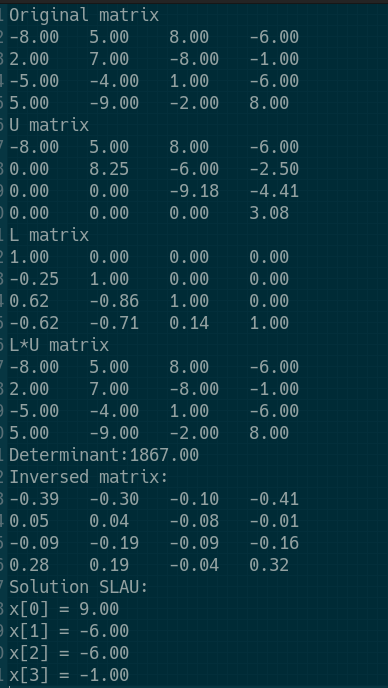
\includegraphics[width=.3\textwidth]{lab1.1}
\caption{Вывод в консоли}
\end{figure}
\pagebreak

\vfill

\subsection{Исходный код}

\lstinputlisting[title=\texttt{1.cpp}]{../stud/svoevolin/exersize_1/1.cpp}
\pagebreak